\newif\ifvimbug
\vimbugfalse

\ifvimbug
\begin{document}
\fi


\subsection{Marching Cubes (3 Punkte)}
\subsubsection{1 Punkt}
Alle blauen Punkte sind innen, alle grünen außen. Die roten Linien sind die eindeutigen Kanten / Zellen und die Zellen mit den orangenen und gelben Linien sind uneindeutig. Hierbei kann entweder orange oder gelb gewählt werden. \\
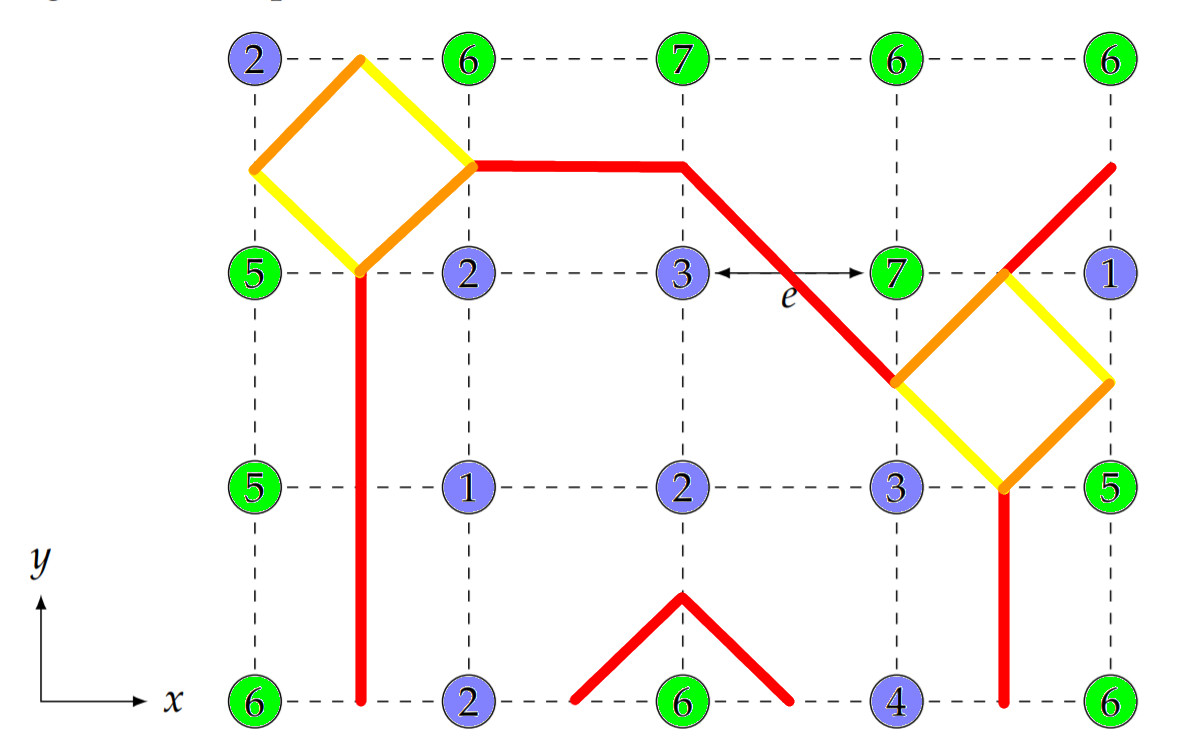
\includegraphics[width=(\textwidth/2)]{51a.jpg} 
\subsubsection{1 Punkt}
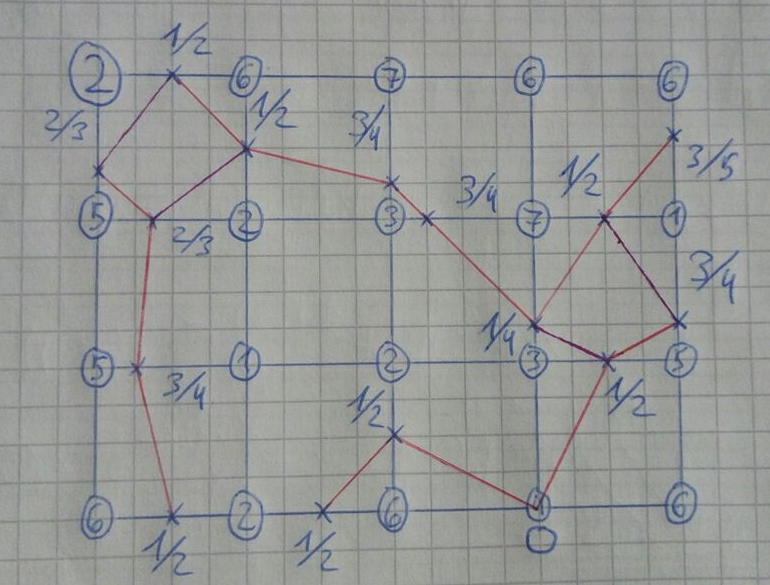
\includegraphics[width=(\textwidth/2)]{1b.png} 
\subsubsection{1 Punkt}

$\nabla f_{2;2} = 1/2 * \binom{7 - 2}{7 - 2} = \binom{5/2}{5/2}$\\
$\nabla f_{3;2} = 1/2 * \binom{1 - 3}{6 - 3} = \binom{-1}{3/2}$\\
$\nabla f_s = 1/4 * \binom{-1}{3/2} + (1 - \frac{1}{4})\binom{5/2}{5/2} = \binom{-1/4}{3/8} + \binom{15/8}{15/8} = \binom{13/8}{18/8} = \binom{1.625}{2.25}$